\begin{chapterenv}

\chapter{Supervised Fine-Tuning \& The Cold Start}

\section{Why SFT Comes First}

\begin{figure}[htbp]
\centering
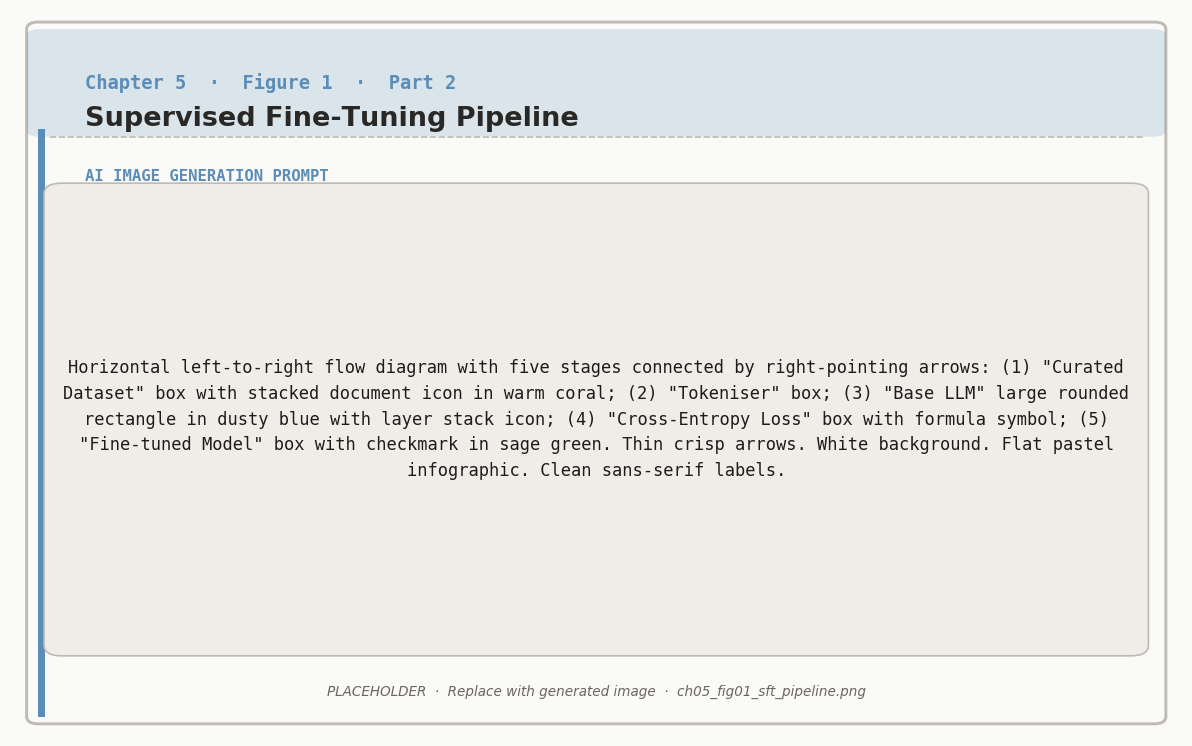
\includegraphics[width=0.92\linewidth]{images/ch05_fig01_sft_pipeline.png}
\caption{The supervised fine-tuning pipeline: curated prompt--response pairs are used to minimise cross-entropy loss on the base LLM.}
\label{fig:ch05:sft}
\end{figure}

In Chapter 2, we identified the alignment gap: language models trained to predict text are not automatically helpful, harmless, or honest. In Chapter 3, we built the RL vocabulary of policies, rewards, and value functions. In Chapter 4, we set up a working environment and verified that the entire training pipeline runs. Now we take the first concrete step toward closing that gap.

That step is \textbf{Supervised Fine-Tuning} (SFT).

The idea is simple. Before a model can improve through trial and error (reinforcement learning), it needs basic competence. Think of it like training a new employee. You would not drop someone into a high-stakes client meeting on their first day and say ``learn from feedback.'' You would first show them how things work: here is how we greet clients, here is how we structure a proposal, here is how we handle complaints. Only after they have internalized the basics does learning-from-feedback become productive.

SFT is that first phase. We show the model thousands of examples of good behavior, and it learns to imitate them. The result is not a perfect model, but it is a model that knows the basic format, tone, and structure of helpful responses. That foundation is what makes everything in Chapters 6 through 12 possible.

But this chapter goes beyond basic SFT. We will also introduce the \textbf{cold start technique}: a way of structuring the training data so that the model learns to \textit{think before it answers}. This single idea, which involves teaching the model to produce internal reasoning traces before giving its final response, is the foundation that the entire reasoning pipeline in Part 3 of this book depends on. Without it, the RL algorithms in later chapters would have nothing to optimize.

\section{The SFT Training Objective}

\subsection{Same Loss, Different Data}

Here is a surprising fact: the SFT loss function is \textit{identical} to the pretraining loss from Chapter 2. Both use negative log-likelihood (next-token prediction). The only difference is the data.

\begin{center}
\begin{tabular}{p{0.20\textwidth}p{0.33\textwidth}p{0.33\textwidth}}
\toprule
& \textbf{Pretraining} & \textbf{SFT} \\
\midrule
Data source & Raw internet text (Reddit, Wikipedia, books, code) & Curated (prompt, response) pairs written or approved by humans \\
Data quality & Mixed: helpful, toxic, wrong, brilliant, all jumbled together & High: every example is a ``good'' response \\
Data volume & Trillions of tokens & Thousands to hundreds of thousands of examples \\
What model learns & How text works in general & How to respond helpfully to specific instructions \\
\bottomrule
\end{tabular}
\end{center}

\begin{tipbox}
SFT uses the same math as pretraining but different data. Pretraining teaches the model how language works. SFT teaches it how a helpful assistant behaves.
\end{tipbox}

\subsection{The Math}

\begin{infobox}
\textbf{The SFT Loss Function}

\begin{center}
\begin{tabular}{p{0.43\textwidth}p{0.43\textwidth}}
\toprule
\textbf{Formal Math} & \textbf{What It Really Means} \\
\midrule
$\mathcal{L}_{\text{SFT}}(\theta) = -\mathbb{E}_{(x,y) \sim \mathcal{D}}\!\left[\sum_{t=1}^T \log \pi_\theta(y_t \,|\, x, y_{<t})\right]$ & Average surprise across all demonstration examples \\
\bottomrule
\end{tabular}
\end{center}

\textbf{What each part means:}

\begin{center}
\begin{tabular}{p{0.35\textwidth}p{0.55\textwidth}}
\toprule
\textbf{Component} & \textbf{Purpose} \\
\midrule
$\mathcal{L}_{\text{SFT}}$ & Loss for Supervised Fine-Tuning \\
$(x, y) \sim \mathcal{D}$ & Sample a (prompt, demonstration) pair from dataset $\mathcal{D}$ \\
$\mathbb{E}[\cdot]$ & Average over all examples (we care about overall performance) \\
$\sum_{t=1}^T$ & For each token position $t$ in the demonstration (1 to $T$), we train on every token \\
$\log \pi_\theta(y_t \,|\, x, y_{<t})$ & Log probability the model assigns to the correct token $y_t$ given the prompt and all previous tokens \\
$-$ (minus sign) & Flip to make it a loss (minimize loss = maximize probability) \\
\bottomrule
\end{tabular}
\end{center}

\textbf{Key detail: prompt masking.} During SFT, we only compute the loss on the \textit{response} tokens, not the prompt tokens. The model sees the prompt as context but is only penalized for getting response tokens wrong. This is different from pretraining, where every token contributes to the loss.
\end{infobox}

\subsection{Step-by-Step Example with Real Numbers}

\textbf{Demonstration from dataset:}
\begin{itemize}[nosep]
    \item \textbf{Prompt ($x$):} ``Explain gravity simply''
    \item \textbf{Good response ($y$):} ``Gravity pulls objects together''
\end{itemize}

This response has $T = 4$ tokens: [``Gravity'', ``pulls'', ``objects'', ``together''].

\paragraph{Position $t=1$: Predict ``Gravity''}

Input to model: ``Explain gravity simply.''

\begin{center}
\begin{tabular}{lcc}
\toprule
\textbf{Token} & \textbf{Probability} & \\
\midrule
``Gravity'' & 0.60 & $\leftarrow$ Correct! \\
``The'' & 0.20 & \\
``It'' & 0.15 & \\
Others & 0.05 & \\
\bottomrule
\end{tabular}
\end{center}

Loss for this token: $-\log(0.60) = 0.51$

\paragraph{Position $t=2$: Predict ``pulls''}

Input to model: ``Explain gravity simply. Gravity''

\begin{center}
\begin{tabular}{lcc}
\toprule
\textbf{Token} & \textbf{Probability} & \\
\midrule
``pulls'' & 0.45 & $\leftarrow$ Correct! \\
``is'' & 0.30 & \\
``attracts'' & 0.15 & \\
Others & 0.10 & \\
\bottomrule
\end{tabular}
\end{center}

Loss: $-\log(0.45) = 0.80$

\paragraph{Position $t=3$: Predict ``objects''}

Input: ``Explain gravity simply. Gravity pulls''

\begin{center}
\begin{tabular}{lcc}
\toprule
\textbf{Token} & \textbf{Probability} & \\
\midrule
``objects'' & 0.70 & $\leftarrow$ Correct! \\
``things'' & 0.20 & \\
``matter'' & 0.08 & \\
Others & 0.02 & \\
\bottomrule
\end{tabular}
\end{center}

Loss: $-\log(0.70) = 0.36$

\paragraph{Position $t=4$: Predict ``together''}

Input: ``Explain gravity simply. Gravity pulls objects''

\begin{center}
\begin{tabular}{lcc}
\toprule
\textbf{Token} & \textbf{Probability} & \\
\midrule
``together'' & 0.55 & $\leftarrow$ Correct! \\
``downward'' & 0.25 & \\
``towards'' & 0.15 & \\
Others & 0.05 & \\
\bottomrule
\end{tabular}
\end{center}

Loss: $-\log(0.55) = 0.60$

\textbf{Total loss for this example:}

\begin{align*}
\mathcal{L}_{\text{this example}} &= \frac{1}{T}\sum_{t=1}^T -\log \pi_\theta(y_t \,|\, x, y_{<t}) \\
&= \frac{1}{4}(0.51 + 0.80 + 0.36 + 0.60) = \frac{2.27}{4} = 0.57
\end{align*}

\textbf{Now average over ALL demonstrations in the dataset:}

\begin{align*}
\mathcal{L}_{\text{SFT}} &= \frac{1}{N} \sum_{\text{all examples}} \mathcal{L}_{\text{example}} \approx 0.62 \quad \text{(average over dataset)}
\end{align*}

\begin{infobox}
\textbf{What gradient descent does with this loss:}

\begin{enumerate}[nosep]
    \item Calculate the loss (0.62)
    \item Compute gradients: ``How should I adjust each parameter to reduce this loss?''
    \item Update the model parameters in the direction that reduces the loss
    \item New loss after one update: 0.58 (improved!)
    \item Repeat for thousands of iterations
    \item Final loss: 0.15 (much better!)
\end{enumerate}

\textbf{Result:} The model learns to generate responses similar to the demonstrations. It has internalized the patterns of what a good response looks like.
\end{infobox}

\section{LoRA: Training on a Budget}

In Chapter 4, we used LoRA to add trainable parameters to our model and promised the math for this chapter. Here it is.

\subsection{The Problem}

Our Qwen2.5-1.5B model has 1.5 billion parameters. Updating all of them during fine-tuning would require storing the model weights, the gradients (same size as the weights), and the optimizer states (typically 2x the weight size for Adam). That adds up to roughly 4x the model size in GPU memory. For a 1.5B model in 16-bit precision, that is about 12 GB just for training state, leaving almost no room on a T4 (15 GB) for the actual data and activations.

\subsection{The LoRA Insight}

The key insight behind LoRA (Low-Rank Adaptation) comes from a 2021 paper by Hu et al. They observed that when you fine-tune a large model, the weight changes tend to be \textit{low-rank}. In plain English: even though the model has billions of parameters, the actual ``meaningful adjustments'' during fine-tuning can be captured by a much smaller number of parameters.

\begin{infobox}
\textbf{LoRA: The Core Idea}

Instead of updating the full weight matrix $W$ (which is enormous), LoRA adds a small trainable ``side path'' that captures the change:

$$W' = W + \Delta W = W + BA$$

\textbf{What each piece means:}

\begin{center}
\begin{tabular}{p{0.25\textwidth}p{0.65\textwidth}}
\toprule
\textbf{Symbol} & \textbf{Meaning} \\
\midrule
$W$ & Original frozen weight matrix (e.g., $4096 \times 4096 = 16.7$ million parameters). Not updated during training. \\
$\Delta W = BA$ & The change we want to learn. Instead of learning all 16.7M entries, decompose into two small matrices. \\
$B$ & Matrix of size $4096 \times r$ (tall and thin) \\
$A$ & Matrix of size $r \times 4096$ (short and wide) \\
$r$ & The \textbf{rank}: typically 8, 16, or 32. Controls how much capacity the adaptation has. \\
$W'$ & Effective weight after adaptation: original + learned change \\
\bottomrule
\end{tabular}
\end{center}

\textbf{Parameter savings with $r = 16$:}

Full update: $4096 \times 4096 = 16{,}777{,}216$ trainable parameters per layer.

LoRA update: $4096 \times 16 + 16 \times 4096 = 65{,}536 + 65{,}536 = 131{,}072$ trainable parameters per layer.

\textbf{That is a 128x reduction!} Across all layers, this means training about 1 to 2\% of the total parameters instead of 100\%.
\end{infobox}

\subsection{Why Does This Work?}

Think of it by analogy. Imagine you have a skilled employee (the pretrained model) who is already very good at their job. You do not need to retrain them from scratch to handle a new type of client. You just need to teach them a few new habits and adjustments. LoRA is exactly that: a small, targeted set of adjustments on top of a strong foundation.

The rank $r$ controls how many ``new habits'' the model can learn. Higher $r$ means more capacity for adaptation, but also more parameters to train and more memory usage. In practice, $r = 16$ is a good default that balances capacity and efficiency.

\begin{tipbox}
In Chapter 4, we set $r = 16$ in \texttt{get\_peft\_model}. That is the rank. The model trained about 1 to 2\% of its parameters. LoRA is why fine-tuning works on a free GPU.
\end{tipbox}

\subsection{Connecting to Code}

Here is the LoRA configuration from Chapter 4, now with annotations explaining each parameter:

\begin{codeblock}[python]
model = FastLanguageModel.get_peft_model(
    model,
    r = 16,                # Rank: capacity of the adaptation
    target_modules = [     # Which weight matrices get LoRA
        "q_proj", "k_proj", "v_proj", "o_proj",  # Attention
        "gate_proj", "up_proj", "down_proj",      # Feed-forward
    ],
    lora_alpha = 16,       # Scaling factor (usually = r)
    lora_dropout = 0,      # No dropout (Unsloth default)
    bias = "none",         # Do not train bias terms
    use_gradient_checkpointing = "unsloth",  # Memory savings
    random_state = 42,
    max_seq_length = max_seq_length,
)
\end{codeblock}

The \texttt{target\_modules} list specifies which weight matrices inside each transformer layer receive LoRA adapters. The attention projections (\texttt{q\_proj}, \texttt{k\_proj}, \texttt{v\_proj}, \texttt{o\_proj}) control how the model attends to different parts of the input. The feed-forward projections (\texttt{gate\_proj}, \texttt{up\_proj}, \texttt{down\_proj}) control how the model transforms representations between attention layers. By adding LoRA to all of these, we give the model flexibility to adapt its behavior across the full transformer stack while keeping memory usage low.

\section{The Cold Start Problem}

Everything up to this point, the SFT loss, LoRA, the training pipeline, is well-established practice. Thousands of tutorials cover it. But there is a deeper problem that most tutorials ignore, and it is the reason this chapter exists as a standalone chapter in this book rather than a footnote.

\subsection{What Happens Without the Cold Start}

\begin{figure}[htbp]
\centering
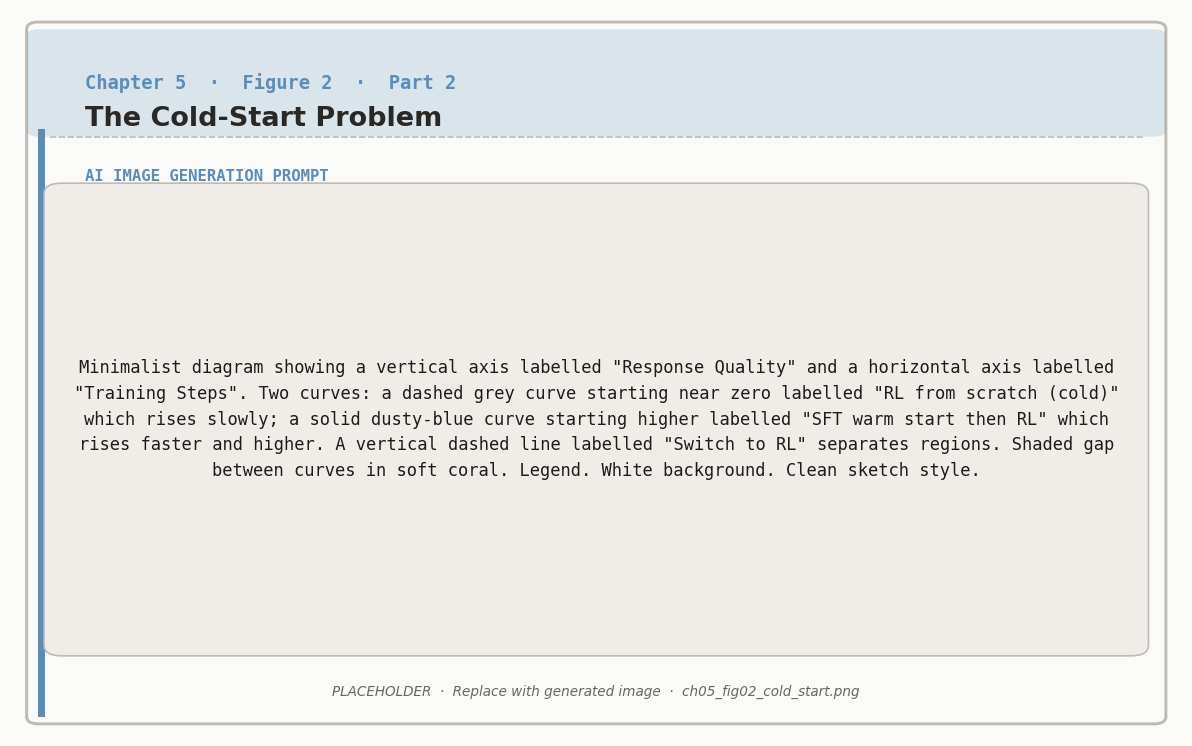
\includegraphics[width=0.92\linewidth]{images/ch05_fig02_cold_start.png}
\caption{The cold-start problem: RL from scratch (dashed) struggles without an initial policy; SFT warm-starting (solid) accelerates learning.}
\label{fig:ch05:coldstart}
\end{figure}

Consider a typical SFT dataset. The training examples look like this:

\begin{center}
\begin{tabular}{p{0.30\textwidth}p{0.60\textwidth}}
\toprule
\textbf{Prompt} & \textbf{Response} \\
\midrule
What is 15\% of 80? & 15\% of 80 is 12. \\
Solve: $2x + 3 = 11$ & $x = 4$. \\
Is 17 prime? & Yes, 17 is a prime number. \\
\bottomrule
\end{tabular}
\end{center}

The model trains on these, and the loss decreases beautifully. After SFT, you test it:

\textbf{Prompt:} ``What is 23\% of 170?''

\textbf{Model output:} ``23\% of 170 is 39.1.''

Correct! But now try something harder:

\textbf{Prompt:} ``A store marks up items by 40\%, then offers a 25\% discount. What is the effective markup?''

\textbf{Model output:} ``The effective markup is 15\%.''

Wrong. The correct answer is 5\% (multiply 1.40 by 0.75 to get 1.05). The model jumped straight to an answer without working through the steps, and it got the reasoning wrong.

\subsection{Why This Happens}

The model learned exactly what the training data taught it: see a math question, output an answer immediately. The demonstrations never showed the model \textit{how to think}. They only showed final answers. So the model has no internal mechanism for multi-step reasoning. It cannot break a problem into steps, work through each one, check its work, and then produce a final answer, because it has never seen that pattern in its training data.

This is the cold start problem. The model arrives at the RL stage (Chapters 6 onward) with no reasoning capability to optimize. RL algorithms like GRPO (Chapter 10) work by generating multiple solution attempts, scoring them, and reinforcing the better ones. But if the model never produces reasoning traces in the first place, there is nothing for the RL algorithm to select from or improve. Every attempt looks the same: a bare answer with no visible thought process.

\begin{infobox}
\textbf{The Cold Start Problem}

\textbf{Without cold start priming:}

RL sees this: ``The answer is 39.1.'' and ``The answer is 41.'' and ``The answer is 39.1.'' All are bare answers. The RL algorithm can score them (right or wrong), but it cannot tell \textit{why} one attempt worked and another failed. There is no reasoning to reinforce or correct.

\textbf{With cold start priming:}

RL sees this: ``Let me think. 23\% means 0.23. Multiply by 170. That gives 39.1. The answer is 39.1.'' Now the RL algorithm can see the reasoning chain. If the model makes a mistake at step 2, a process reward model (Chapter 9) can identify exactly where things went wrong. GRPO (Chapter 10) can reinforce good reasoning chains and suppress bad ones.

\textbf{The cold start technique gives RL something to work with.} Without it, RL is blind.
\end{infobox}

\section{The Solution: Think Tag Priming}

The solution is elegant. Instead of training on bare answers, we structure the SFT data so that every response includes an explicit reasoning trace wrapped in special tags.

\subsection{The Format}

The format uses a \texttt{<think>} tag to separate the model's internal reasoning from its final answer:

\begin{codeblock}[python]
# Training example WITHOUT cold start (bare answer)
{"role": "user", "content": "What is 23% of 170?"}
{"role": "assistant", "content": "23% of 170 is 39.1."}

# Training example WITH cold start (think-tag priming)
{"role": "user", "content": "What is 23% of 170?"}
{"role": "assistant", "content":
    "<think>\n"
    "I need to calculate 23% of 170.\n"
    "23% as a decimal is 0.23.\n"
    "0.23 multiplied by 170:\n"
    "0.23 * 170 = 0.23 * 100 + 0.23 * 70\n"
    "= 23 + 16.1\n"
    "= 39.1\n"
    "</think>\n"
    "23% of 170 is 39.1."}
\end{codeblock}

The model learns two things simultaneously: (1) when given a question, produce a \texttt{<think>} block first, and (2) inside that block, break the problem into explicit steps before giving the final answer.

\subsection{Why This Works}

The \texttt{<think>} tag approach works for three reasons that reinforce each other.

\textbf{First, it exploits the model's autoregressive nature.} A language model generates text left to right, one token at a time. Each token it generates becomes part of the context for the next token. When the model writes ``23\% as a decimal is 0.23'' inside a think block, that intermediate result is now in the context window. The model can ``see'' its own work and use it for the next step. Without the think block, the model must do all the reasoning implicitly in its hidden states, which is far less reliable for multi-step problems.

\textbf{Second, it creates a structured signal for RL.} Once the model produces reasoning traces, later RL stages (Chapters 10 through 12) can evaluate and optimize those traces. A process reward model (Chapter 9) can score individual reasoning steps. GRPO (Chapter 10) can compare different reasoning chains for the same problem and reinforce the better ones. None of this is possible if the model only outputs bare answers.

\textbf{Third, it is cheap.} Generating think-tag training data is straightforward. For math and code problems, you can use a stronger model (like GPT-4 or Gemini) to generate step-by-step solutions, then format them with think tags. For many domains, you can use existing chain-of-thought datasets. The cold start does not require human annotation of reasoning steps. It just requires that the training data include reasoning in a structured format.

\begin{infobox}
\textbf{Think of it like teaching a student to show their work.}

A math teacher does not just check final answers. They require students to write out each step. Not because the steps are the goal (the correct answer is), but because showing work (a) forces the student to actually reason through the problem, (b) lets the teacher identify where mistakes happen, and (c) builds a habit of careful thinking that transfers to harder problems.

The \texttt{<think>} tag serves the same purpose for the model. It forces explicit reasoning, makes that reasoning visible to reward signals, and builds a pattern that RL can later optimize.
\end{infobox}

\subsection{What the Training Data Looks Like}

Here are several examples showing how different types of problems get formatted with think tags. Notice that the reasoning style adapts to the problem type:

\begin{codeblock}[python]
# Math reasoning
{
    "messages": [
        {"role": "user", "content":
         "A store marks up items by 40%, then offers a 25% "
         "discount. What is the effective markup?"},
        {"role": "assistant", "content":
         "<think>\n"
         "Start with a base price of $100.\n"
         "After 40% markup: $100 * 1.40 = $140.\n"
         "After 25% discount: $140 * 0.75 = $105.\n"
         "Effective markup: ($105 - $100) / $100 = 5%.\n"
         "The markups do not simply subtract because "
         "the discount applies to the marked-up price, "
         "not the original.\n"
         "</think>\n"
         "The effective markup is 5%."}
    ]
}
\end{codeblock}

\begin{codeblock}[python]
# Logical reasoning
{
    "messages": [
        {"role": "user", "content":
         "All roses are flowers. Some flowers fade quickly. "
         "Can we conclude that some roses fade quickly?"},
        {"role": "assistant", "content":
         "<think>\n"
         "Premise 1: All roses are flowers.\n"
         "Premise 2: Some flowers fade quickly.\n"
         "Question: Do some roses fade quickly?\n"
         "The flowers that fade quickly might or might not "
         "include roses. Premise 2 says SOME flowers fade "
         "quickly, but does not specify which ones.\n"
         "This is the fallacy of the undistributed middle.\n"
         "We cannot conclude this.\n"
         "</think>\n"
         "No, we cannot conclude that. While all roses are "
         "flowers, the flowers that fade quickly might be "
         "entirely non-rose flowers. The premises do not "
         "give us enough information to draw that conclusion."}
    ]
}
\end{codeblock}

\begin{codeblock}[python]
# Simple factual question (minimal think block)
{
    "messages": [
        {"role": "user", "content": "What is the capital of France?"},
        {"role": "assistant", "content":
         "<think>\n"
         "This is a straightforward factual question.\n"
         "</think>\n"
         "The capital of France is Paris."}
    ]
}
\end{codeblock}

\begin{tipbox}
Even simple questions get a think block, even if it is brief. This teaches the model the consistent habit of always reasoning first, regardless of difficulty.
\end{tipbox}

\section{Hands-On: Your First Real SFT Run}

Now we put everything together. We will use the environment from Chapter 4, load a proper dataset with think-tag formatting, and run a real SFT training session.

\subsection{Step 1: Load the Model (Same as Chapter 4)}

\begin{codeblock}[python]
from unsloth import FastLanguageModel
import torch

max_seq_length = 2048
model_name = "unsloth/Qwen2.5-1.5B-Instruct"

model, tokenizer = FastLanguageModel.from_pretrained(
    model_name = model_name,
    max_seq_length = max_seq_length,
    load_in_4bit = True,
    load_in_8bit = False,
)

# Add LoRA adapters (r=16, same as Chapter 4)
model = FastLanguageModel.get_peft_model(
    model,
    r = 16,
    target_modules = [
        "q_proj", "k_proj", "v_proj", "o_proj",
        "gate_proj", "up_proj", "down_proj",
    ],
    lora_alpha = 16,
    lora_dropout = 0,
    bias = "none",
    use_gradient_checkpointing = "unsloth",
    random_state = 42,
    max_seq_length = max_seq_length,
)
\end{codeblock}

\subsection{Step 2: Prepare the Dataset with Think Tags}

For this hands-on exercise, we will create a dataset of 50 examples with think-tag formatting. In a production setting, you would use thousands of examples, often generated by a stronger model and then filtered for correctness. Here, 50 is enough to demonstrate the technique and see the model learn the think-tag pattern.

\begin{codeblock}[python]
from datasets import Dataset

# Helper function to format a single example
def make_example(question, thinking, answer):
    return {
        "messages": [
            {"role": "user", "content": question},
            {"role": "assistant", "content":
             f"<think>\n{thinking}\n</think>\n{answer}"}
        ]
    }

# Build a dataset with think-tag formatted examples
train_data = [
    make_example(
        "What is 15% of 200?",
        "15% as a decimal is 0.15.\n"
        "0.15 * 200 = 30.",
        "15% of 200 is 30."
    ),
    make_example(
        "Solve: 3x + 7 = 22",
        "Subtract 7 from both sides: 3x = 15.\n"
        "Divide both sides by 3: x = 5.",
        "x = 5."
    ),
    make_example(
        "Is 51 a prime number?",
        "Check divisibility. 51 / 3 = 17.\n"
        "Since 51 = 3 * 17, it is not prime.",
        "No, 51 is not prime. It equals 3 times 17."
    ),
    make_example(
        "What is the sum of the first 10 positive integers?",
        "Use the formula: n(n+1)/2.\n"
        "n = 10, so 10 * 11 / 2 = 55.",
        "The sum is 55."
    ),
    make_example(
        "A train travels 120 km in 1.5 hours. "
        "What is its average speed?",
        "Speed = distance / time.\n"
        "Speed = 120 / 1.5 = 80 km/h.",
        "The average speed is 80 km/h."
    ),
    # ... (in practice, include 45 more examples covering
    #  math, logic, coding, and general knowledge)
]

# For this demonstration, duplicate and vary examples
# to reach 50 training samples
import copy
while len(train_data) < 50:
    for item in list(train_data):
        if len(train_data) >= 50:
            break
        train_data.append(copy.deepcopy(item))

dataset = Dataset.from_list(train_data)
print(f"Dataset size: {len(dataset)} examples")
\end{codeblock}

\begin{infobox}
\textbf{Where do real think-tag datasets come from?}

For production SFT, there are several sources:

\textbf{Distillation from stronger models.} Send your prompts to a model like GPT-4o or Claude and ask it to ``think step by step, wrapping your reasoning in <think> tags.'' Filter the results for correctness, then use them as training data. This is the most common approach in practice.

\textbf{Existing chain-of-thought datasets.} Datasets like OpenMathInstruct, MetaMathQA, and Orca-Math already contain step-by-step solutions. You just need to reformat them with think tags.

\textbf{Human annotation.} More expensive but higher quality. Have domain experts write reasoning traces for problems in your target domain. Best for specialized applications.

For the exercises in this book, we will use small hand-crafted datasets to keep things runnable on free GPUs. The technique itself scales to any dataset size.
\end{infobox}

\subsection{Step 3: Configure and Run the Trainer}

\begin{codeblock}[python]
from trl import SFTTrainer, SFTConfig

trainer = SFTTrainer(
    model = model,
    tokenizer = tokenizer,
    train_dataset = dataset,
    args = SFTConfig(
        per_device_train_batch_size = 2,
        gradient_accumulation_steps = 4,
        warmup_steps = 10,
        max_steps = 100,           # More steps than Ch 4
        learning_rate = 2e-4,
        logging_steps = 10,
        output_dir = "sft_outputs",
        optim = "adamw_8bit",
        seed = 42,
        report_to = "none",
        max_seq_length = max_seq_length,
    ),
)

print("Starting SFT training with think-tag data...")
stats = trainer.train()
print(f"Training complete! Final loss: {stats.training_loss:.4f}")
\end{codeblock}

This will take approximately 3 to 5 minutes on a free T4 GPU. Watch the loss values as they are logged every 10 steps. You should see the loss decrease steadily, indicating the model is learning the think-tag response pattern.

\subsection{Step 4: Test the Cold-Started Model}

Now for the moment of truth. Does the model produce think blocks?

\begin{codeblock}[python]
# Switch to inference mode
FastLanguageModel.for_inference(model)

from transformers import TextStreamer

# Test with a question similar to training data
test_prompts = [
    "What is 30% of 250?",
    "Solve: 5x - 3 = 22",
    "A car travels 200 km in 2.5 hours. "
    "What is its average speed?",
]

for prompt in test_prompts:
    print(f"\n{'='*50}")
    print(f"PROMPT: {prompt}")
    print(f"{'='*50}")
    messages = [{"role": "user", "content": prompt}]
    inputs = tokenizer.apply_chat_template(
        messages,
        tokenize = True,
        add_generation_prompt = True,
        return_tensors = "pt",
    ).to("cuda")
    _ = model.generate(
        input_ids = inputs,
        max_new_tokens = 512,
        temperature = 0.7,
        streamer = TextStreamer(tokenizer),
    )
\end{codeblock}

If the training worked, you should see responses that begin with \texttt{<think>}, contain step-by-step reasoning, close with \texttt{</think>}, and then give a final answer. Even with only 50 examples and 100 training steps, the model typically picks up the think-tag pattern. The quality of the reasoning may be rough, but the \textit{structure} is there. And the structure is what matters for the cold start, because RL will optimize the reasoning quality later.

\begin{tipbox}
Do not worry if the reasoning inside the think blocks is sometimes wrong at this stage. SFT teaches format and pattern, not perfect reasoning. Perfecting the reasoning is what RL does in Chapters 10 through 12.
\end{tipbox}

\section{Evaluating SFT Quality}

How do you know if your SFT run was successful? There are three levels of evaluation, from quick checks to systematic analysis.

\subsection{Level 1: Loss Curves}

The most basic check is whether the training loss decreased. A healthy SFT run typically shows:

\begin{center}
\begin{tabular}{lcc}
\toprule
\textbf{Pattern} & \textbf{What It Means} & \textbf{Action} \\
\midrule
Loss decreases smoothly & Training is working & Continue \\
Loss plateaus early & Learning rate may be too low, or data is too easy & Increase LR or add harder examples \\
Loss oscillates wildly & Learning rate too high or batch size too small & Decrease LR or increase batch \\
Loss increases & Something is wrong (data format, LR too high) & Debug immediately \\
\bottomrule
\end{tabular}
\end{center}

\subsection{Level 2: Qualitative Spot Checks}

Run the model on 10 to 20 test prompts and inspect the outputs manually. For think-tag SFT, check for three things:

\textbf{Format compliance.} Does every response start with \texttt{<think>} and include a \texttt{</think>} before the final answer? If the model sometimes forgets the tags or produces malformed output, you may need more training steps or more diverse examples.

\textbf{Reasoning structure.} Inside the think block, does the model break the problem into steps, or does it just restate the question? Good: ``First, convert 23\% to 0.23. Then multiply by 170.'' Bad: ``I need to figure out 23\% of 170. The answer is 39.1.''

\textbf{Answer correctness on easy problems.} For problems similar to the training data, does the model get the right answer? SFT alone will not make the model perfect on hard problems, but it should handle straightforward ones. If it fails on easy problems, the training data quality may be the issue.

\subsection{Level 3: Systematic Evaluation}

For a more rigorous check, you can compute accuracy on a held-out set:

\begin{codeblock}[python]
# Simple evaluation: check if model produces think tags
# and correct answers on held-out examples
eval_prompts = [
    ("What is 12% of 300?", "36"),
    ("Solve: 4x = 28", "7"),
    ("Is 29 prime?", "yes"),
]

correct = 0
has_think_tags = 0

for prompt, expected in eval_prompts:
    messages = [{"role": "user", "content": prompt}]
    inputs = tokenizer.apply_chat_template(
        messages,
        tokenize = True,
        add_generation_prompt = True,
        return_tensors = "pt",
    ).to("cuda")
    output_ids = model.generate(
        input_ids = inputs,
        max_new_tokens = 512,
        temperature = 0.1,  # Low temp for evaluation
    )
    response = tokenizer.decode(
        output_ids[0][inputs.shape[1]:],
        skip_special_tokens = True
    )

    if "<think>" in response and "</think>" in response:
        has_think_tags += 1
    if expected.lower() in response.lower():
        correct += 1

print(f"Think-tag compliance: {has_think_tags}/{len(eval_prompts)}")
print(f"Answer accuracy: {correct}/{len(eval_prompts)}")
\end{codeblock}

\begin{tipbox}
Use low temperature (0.1) during evaluation so results are reproducible. Use higher temperature (0.7 or above) during RL training so the model explores diverse reasoning paths.
\end{tipbox}

\section{What SFT Cannot Do (And Why We Need RL)}

SFT is powerful but limited. Understanding its boundaries is essential for understanding why the rest of this book exists.

\subsection{SFT Only Imitates}

SFT teaches the model to reproduce patterns from its training data. If the training data contains a particular style of reasoning, the model will imitate that style. But it cannot \textit{improve} beyond the demonstrations. If the training data solves a problem in a roundabout way, the model will learn that roundabout approach. It has no mechanism to discover that a more direct solution exists.

\subsection{SFT Cannot Generalize Reasoning}

The model learns surface patterns of reasoning, not deep understanding. It might learn that ``divide both sides by 2'' follows ``2x = 8'' because that pattern appeared many times. But it does not truly understand \textit{why} division is the right operation. When faced with a novel problem structure it has never seen, the imitated reasoning may fail.

\subsection{SFT Is Bounded by Data Quality}

If the training demonstrations contain subtle errors, biases, or suboptimal approaches, the model faithfully learns those flaws. There is no built-in mechanism for the model to recognize or correct mistakes in its training data. It treats every demonstration as equally valid.

\begin{infobox}
\textbf{The SFT ceiling, illustrated}

Imagine you learn cooking by watching exactly 100 recipe videos. After watching them, you can reproduce those 100 dishes fairly well. But:

You cannot invent new dishes (limited to what you have seen).

You cannot improve on the recipes (if the video used too much salt, you will too).

You cannot adapt when ingredients change (you learned specific patterns, not general principles).

\textbf{What you need next:} Actual practice in a kitchen, with someone tasting your food and telling you what works. That is RL.

SFT gives us a model that produces structured reasoning traces in a consistent format. RL (Chapters 6 through 12) takes that foundation and optimizes the \textit{quality} of the reasoning itself.
\end{infobox}

\subsection{The Roadmap from Here}

Here is where each limitation gets addressed in the chapters ahead:

\begin{center}
\begin{tabular}{p{0.35\textwidth}p{0.15\textwidth}p{0.35\textwidth}}
\toprule
\textbf{SFT Limitation} & \textbf{Addressed in} & \textbf{How} \\
\midrule
Cannot improve beyond demonstrations & Chapter 6 & PPO optimizes responses using reward signal \\
Bounded by data quality & Chapter 7 & DPO learns from preference pairs without a reward model \\
No mechanism to evaluate own reasoning & Chapter 9 & Process reward models score individual steps \\
Cannot discover better reasoning strategies & Chapter 10 & GRPO reinforces high-quality reasoning chains \\
Cannot verify its own answers & Chapter 11 & Verifiers and RLVR provide automated correctness checks \\
\bottomrule
\end{tabular}
\end{center}

\section{What We Built and What Comes Next}

In this chapter, we accomplished three things.

\textbf{First}, we understood the SFT training objective: the same next-token prediction loss as pretraining, but applied to curated demonstration data. We walked through the math with real numbers and connected it to the gradient descent process.

\textbf{Second}, we understood LoRA: the technique that makes fine-tuning possible on free GPUs by decomposing weight updates into small, low-rank matrices. The $W' = W + BA$ decomposition reduces trainable parameters by roughly 128x.

\textbf{Third}, and most importantly, we solved the cold start problem. By formatting our SFT data with \texttt{<think>} tags, we taught the model to produce explicit reasoning traces before answering. This gives the RL algorithms in later chapters something concrete to optimize.

The model we have built is competent but imperfect. It follows instructions, it produces reasoning traces, and it gets easy problems right. But it is still limited to imitating its training data. It cannot improve beyond what it has seen, and its reasoning on hard problems is unreliable.

In the next chapter, we will break through that ceiling. Chapter 6 introduces reward models and PPO, the first technique that lets the model improve \textit{beyond} its demonstrations by learning from human preferences. The cold-started model we built here is exactly the starting point that PPO needs.

The foundation is set. Now the real training begins.


\begin{tipbox}
\textbf{Companion notebook.} The code for this chapter is in
\texttt{code/notebooks/part2\_core/05\_sft.ipynb}
in the book repository at \texttt{github.com/arunpshankar/packt-final}.
On GitHub, navigate to the file and replace \texttt{github.com} with
\texttt{githubtocolab.com} in the URL to open it directly in Colab.
\end{tipbox}

\end{chapterenv}